\documentclass[12pt, titlepage]{article}

% For formatting
\usepackage[margin=1truein]{geometry}
\usepackage{fancyhdr}
\usepackage{setspace}
\usepackage{titlesec}
\usepackage{graphicx}
\usepackage{float}
\usepackage{color}
\usepackage{listings}
\usepackage{cite}

% For equations
\usepackage{amsmath, amssymb}
\usepackage{physics}
\usepackage{newtxtext, newtxmath}

\newcommand{\mytitle}{Numerical Solutions to Elliptical Partial Differential Equations}

\definecolor{verbgray}{gray}{0.9}

% New code environment that is just the verbatim environment with color bg
\lstnewenvironment{code}{
    \lstset{backgroundcolor=\color{verbgray},
    frame=single,
    framerule=0pt,
    basicstyle=\ttfamily,
    columns=fullflexible}
}{}

\definecolor{shadecolor}{rgb}{.9, .9, .9}

\title{\mytitle}
\author{Jaden Nola}
\date{2 May 2023}

\pagestyle{fancy}
\fancyhf{}
\fancyhead[C]{\mytitle}
\fancyhead[R]{\thepage}
\renewcommand{\headrulewidth}{0pt}
\setlength{\headheight}{15pt}

\setlength{\parskip}{\lineskip}
\titleformat{\section}{\normalfont\fontsize{15.6}{15.6}\bfseries}{\thesection}{1em}{}
\titlespacing{\section}{0pt}{\parskip}{-\parskip}
\titleformat{\subsection}{\normalfont\fontsize{13.2}{13.2}\bfseries}{\thesubsection}{1em}{}
\titlespacing{\subsection}{0pt}{\parskip}{-\parskip}

\doublespacing
\begin{document}
    \maketitle
    \section{Background}
    According to Greenbaum~\&~Chartier~\cite{greenbaum}, a \textbf{partial differential equation} (PDE) is an expression which can be written
    in the following form:
    \begin{equation}\label{eq:pde}
        au_{xx} + 2bu_{xy} + cu_{yy} + du_{x} + eu_{y} + fu = g
    \end{equation}
    where \textit{a}, \textit{b}, \textit{c}, \textit{d}, \textit{e}, \textit{f}, and \textit{g} are functions of \textit{x} and \textit{y}.
    From this form, we are able to further classify different types of PDEs based on a quantity known as
    the \textbf{discriminant}. It is defined as
    \begin{equation}
        D \equiv b^2 - ac
    \end{equation}
    When $D < 0$, we say that the equation is \textbf{elliptical}; if $D > 0$, then it is \textbf{hyperbolic}; 
    otherwise, if $D = 0$, then the equation is \textbf{parabolic}. As \textit{a}, \textit{b}, and \textit{c} are functions of \textit{x} and \textit{y},
    the type of PDE represented by Equation~(\ref{eq:pde}) can change types throughout the domain of the solution function.
    This paper will focus on numerical solutions to differential equations to elliptical PDEs.  
    \section{Problem Statement}
    In this paper, we will specifically focus on the \textbf{Poisson~equation}~\cite{burden_faires_2011}, which is given by
    \begin{equation}\label{eq:poisson}
        \grad^2 u(x,y) \equiv \pdv[2]{u}{x}~(x,y) + \pdv[2]{u}{y}~(x,y) = f(x,y)
    \end{equation}
    where $\grad = \text{grad}f = \hat{\imath}\pdv{x} + \hat{\jmath}\pdv{y}$ and $\grad^2 = \grad \cdot \grad = \hat{\imath}\pdv[2]{x} + \hat{\jmath}\pdv[2]{y}$.
    In the case that Equation~(\ref{eq:poisson}) is homogenous (i.e., $f(x,y)=0$), then
    \begin{equation}\label{eq:laplace}
        \grad^2 u(x,y) = 0
    \end{equation}
    and Equation~(\ref{eq:laplace}) is called the \textbf{Laplace~equation}. Observe that since $b = 0$ and $a = c = 1$, 
    the discriminant of Equation~(\ref{eq:poisson}) is $D=-1$, thus the Poisson equation is always elliptic in any domain.

    Our goal is to approximate the solution to this PDE on the open rectangle 
    \begin{equation*}
        R = \left\{(x,y)\; |\; a < x < b,\; c < y < d\right\} \subset \mathbb{R}^2
    \end{equation*}
    Furthermore, we are also subject to boundary conditions $u(x,y) = g(x,y)\;\forall\:(x,y)\in S$, where \textit{S} is
    the boundary of the rectangle \textit{R}. If we have that \textit{f} and \textit{g} are continuous on \textit{R}, then 
    we are guaranteed a unique solution to Equation~(\ref{eq:poisson}).
    \section{Method}
    This section will outline the method described in \cite{burden_faires_2011}. Similar to our methods of approximating linear ordinary differential equations, we will split our rectangle into
    $n+1$ subintervals along the \textit{x}-direction and $m+1$ subintervals of equal length along the \textit{y}-direction, where $m,n \in \mathbb{N}$.
    Thus, we define $h=(b-a)/n$ and $k=(d-c)/m$, which gives $x_i = a  + ih,\; i=0,1,\dots,n$ and $y_j = c + kj, \; k=0,1,\dots,m$. These $(n+1)(m+1)$ points
    form the border and intersections of our \textbf{grid}. In our grid, there are $(n-1)(m-1)$ points that do not lie on the border, which we will call \textbf{mesh points}.

    We assume that our solution function $u(x,y) \in C^4~(R)$, meaning that the fourth derivative is continuous on \textit{R}. In order to find an appropriate approximation to Equation~(\ref{eq:poisson}),
    we apply Taylor's theorem in the \textit{x}-direction. Carrying out this procedure around each mesh point $x_i$,\\
    $i=1,2,\dots,n-1$, we find
    \small
    \begin{align*}
        u(x_i + h, y_j) &= u(x_i, y_j) + \pdv{u}{x}~(x_i,y_j)h+\frac{1}{2!}\pdv[2]{u}{x}~(x_i,y_j)h^2+\frac{1}{3!}\pdv[3]{u}{x}~(x_i,y_j)h^3+\frac{1}{4!}\pdv[4]{u}{x}~(\xi_i,y_j)h^4\\
        u(x_i - h, y_j) &= u(x_i, y_j) - \pdv{u}{x}~(x_i,y_j)h+\frac{1}{2!}\pdv[2]{u}{x}~(x_i,y_j)h^2-\frac{1}{3!}\pdv[3]{u}{x}~(x_i,y_j)h^3+\frac{1}{4!}\pdv[4]{u}{x}~(\eta_i,y_j)h^4
    \end{align*}
    \normalsize
    where $\xi_i \in (x_i, x_i+h)$ and $\eta_i \in (x_i-h,x_i)$. Adding the two equations together, we find
    \small
    \begin{equation*}
        u(x_i + h, y_j) + u(x_i - h, y_j) = 2u(x_i, y_j) + \pdv[2]{u}{x}~(x_i, y_j)h^2 + \frac{h^4}{4!}\left[\pdv[4]{u}{x}~(\xi_i, y_j) + \pdv[4]{u}{x}~(\eta_i, y_j)\right]
    \end{equation*}
    \normalsize
    Without loss of generality, we assume $\pdv[4]{u}{x}~(\xi_i, y_j) \leq \pdv[4]{u}{x}~(\eta_i, y_j)$. Since $\pdv[4]{u}{x}~(x,y)$ is continuous and
    \begin{equation*}
        \pdv[4]{u}{x}~(\xi_i, y_j) \leq \frac{\pdv[4]{u}{x}~(\xi_i, y_j) + \pdv[4]{u}{x}~(\eta_i, y_j)}{2} \leq \pdv[4]{u}{x}~(\eta_i, y_j),
    \end{equation*}
    by the Intermediate Value theorem, there exists $\theta_i \in (x_i - h, x_i + h)$ such that
    \begin{equation*}
        2\pdv[4]{u}{x}~(\theta_i, y_j) = \pdv[4]{u}{x}~(\xi_i, y_j) + \pdv[4]{u}{x}~(\eta_i, y_j)
    \end{equation*}
    Rearranging for the second-derivative, we arrive at the \textbf{centered-difference} formula for the second derivative:
    \begin{equation}\label{eq:x_centered_diff}
        \pdv[2]{u}{x}~(x_i, y_j) = \frac{u(x_i + h, y_j) - 2u(x_i, y_j) + u(x_i - h, y_j)}{h^2} - \frac{h^2}{12}\pdv[4]{u}{x}~(\theta_i, y_j)
    \end{equation}
    Following the same procedure, we can also come up with a centered-difference formula for the second partial derivative in the \textit{y}-direction:
    \begin{equation}\label{eq:y_centered_diff}
        \pdv[2]{u}{y}~(x_i, y_j) = \frac{u(x_i, y_j + k) - 2u(x_i, y_j) + u(x_i, y_j-k)}{k^2} - \frac{k^2}{12}\pdv[4]{u}{y}~(x_i, \phi_j)
    \end{equation}
    with $\phi \in (y_j-k,y_j+k)$. Equations~(\ref{eq:x_centered_diff})~and~(\ref{eq:y_centered_diff}) can be used in Equation~(\ref{eq:poisson}) to give
    \begin{equation}\label{eq:approx_poisson}
        \begin{split}
            &\frac{u(x_i + h, y_j) - 2u(x_i, y_j) + u(x_i - h, y_j)}{h^2} + \frac{u(x_i, y_j + k) - 2u(x_i, y_j) + u(x_i, y_j-k)}{k^2}\\
            &= f(x,y) + \frac{h^2}{12}\pdv[4]{u}{x}~(\theta_i, y_j) + \frac{k^2}{12}\pdv[4]{u}{y}~(x_i, \phi_j)
        \end{split}
    \end{equation}
    with our boundary conditions being
    \begin{equation}\label{eq:bound_conds}
        \begin{split}
            u(x_0, y_j) = g(x_0, y_j)&\text{ and }u(x_n, y_j) = g(x_n, y_j) \;\forall\;j=0,1,\dots,m\\
            u(x_i, y_0) = g(x_i, y_0)&\text{ and }u(x_i, y_m) = g(x_i, y_m) \;\forall\;i=0,1,\dots,n
        \end{split}
    \end{equation}
    This ensures that our numerical solution is correct along the borders of our rectangle \textit{R}.

    A rearrangement of Equation~(\ref{eq:approx_poisson}) yields the following:
    \begin{equation}\label{eq:pde_finite_diff}
        2\left[\left(\frac{h}{k}\right)^2 + 1\right]w_{ij} - (w_{i+1,j} + w_{i-1,j})-\left(\frac{h}{k}\right)^2 (w_{i,j+1}+w_{i,j-1}) = -h^2f(x,y)
    \end{equation}
    where $w_{ij}\approx u(x_i, y_j)$. It follows that our boundary conditions from Equation~(\ref{eq:bound_conds}) becomes
    \begin{align*}
        w_{0j} = g(x_0, y_j)&\text{ and }w_{nj} = g(x_n, y_j) \;\forall\;j=0,1,\dots,m\\
        w_{i0} = g(x_i, y_0)&\text{ and }w_{im} = g(x_i, y_m) \;\forall\;i=0,1,\dots,n
    \end{align*}
    Since we used the centered-difference formula twice, this method has an error of $O(h^2 + k^2)$.

    It is desirable to relabel the mesh points for notational convenience. In particular, we will use the following map of $\mathbb{N}^2 \to \mathbb{N}$:
    \begin{equation}
        P(i,j) = (m-1)(i-1) + j
    \end{equation} 
    for $i=1,2,\dots,n-1$ and $j=1,2,\dots,m-1$. Intuitively, we are counting the mesh points from left to right and top to bottom, as seen in Figure~(\ref{fig:intuitive_grid}).
    \begin{figure}[H]
        \centering
        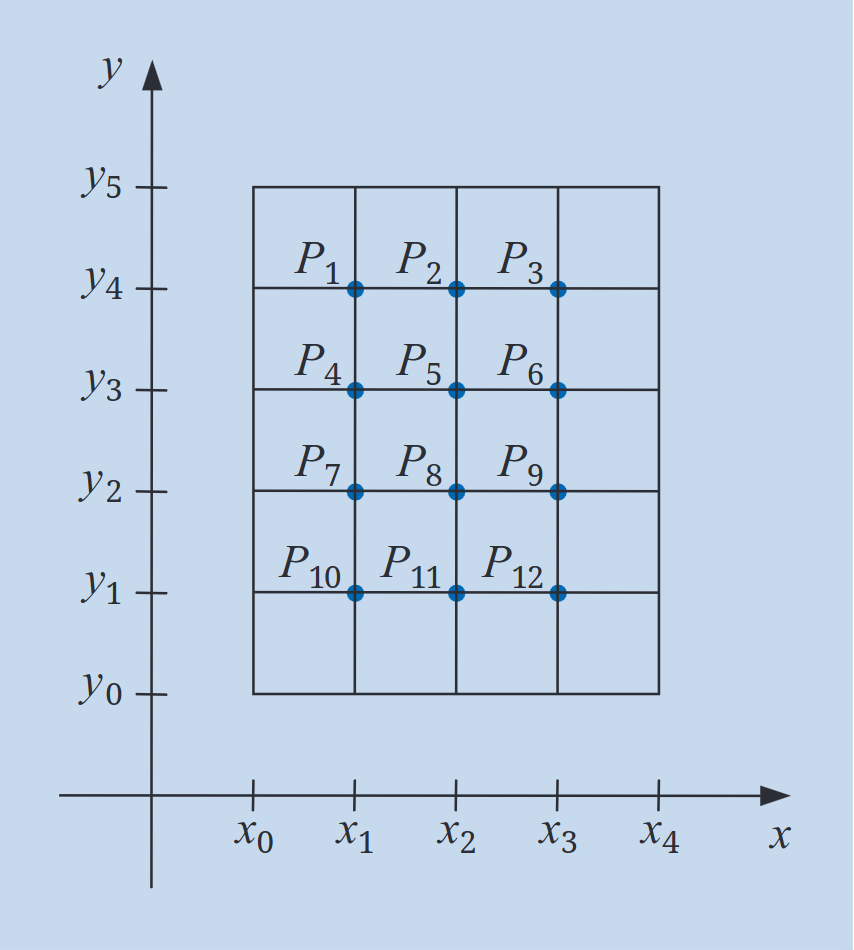
\includegraphics[width=0.4\linewidth]{intuitive_grid.png}
        \caption{Visualization of counting mesh points, from~\cite{burden_faires_2011}}\label{fig:intuitive_grid}
    \end{figure}
    This new labeling convention allows us to relabel our points $w_{ij} = w_l$. Finally, Equation~(\ref{eq:pde_finite_diff}) with $i=1,2,\dots,n-1$ and $j=1,2,\dots,m-1$
    gives us a system of $(n-1)(m-1)$ equations with $(n-1)(m-1)$ unknowns, which can be solved using Gaussian elimination or other techniques. A sample MATLAB implementation
    has been given in Appendix A.
    \section{Results}
    \subsection{Example 1}
    Our first problem will be to find the steady state heat distribution of a thin square metal plate, the solution of which is given by Equation~(\ref{eq:laplace}), the Laplace equation.
    For convenience, we will take our region to be $R = \left\{(x,y)\; |\; 0 \leq x \leq 0.5,\;0\leq y \leq 0.5\right\}$. The boundary conditions are as follows:
    \begin{itemize}
        \item Two adjacent side
    \end{itemize}
    \newpage
    \section*{Appendix A\@: MATLAB Implementation}
    {\singlespacing
        \begin{code}
function [xdisp, ydisp, u] = myPoisson(f, g, a, b, c, d, n, m)
    % Return numerical solutions of the Poisson PDE at mesh points.
    % The PDE is of the form $u_{xx} + u_{yy} = f(x,y)$
    %
    % Params:
    % f - Function that takes in two arguments
    % g - Function that provides B.C. along x=a, x=b, y=c, y=d
    % a - Left bound of rectangle
    % b - Right bound of rectangle
    % c - Lower bound of rectangle
    % d - Upper bound of rectangle
    %
    % Returns a table of the approximated solutions of u at (x,y)
    if (a > b) || (c > d)
        error("Invalid rectangle bounds.")
    end
    if (n < 1) || (m < 1)
        error("Invalid value for n or m.")
    end
    h=(b-a)/n; k=(d-c)/m;
    x = (a:h:b)'; y = (c:k:d)';
    num_side = (n-1)*(m-1);
    xdisp = zeros(num_side, 1);
    ydisp = zeros(num_side, 1);
    u = zeros(num_side, 1);
    coeffs = zeros(num_side);
    b = zeros(num_side, 1);
    b(index(1,1:m-1)) = b(index(1,1:m-1))+g(x(1),y(2:m));
    b(index(1:n-1,1)) = b(index(1:n-1,1))+(((h/k)^2)*g(x(2:n),y(1)));
    b(index(n-1,1:m-1)) = b(index(n-1,1:m-1))+g(x(n+1), y(2:m));
    b(index(1:n-1,m-1)) = b(index(1:n-1,m-1))+(((h/k)^2)*g(x(2:n),y(m+1)));
    row = 1;
    for i=1:n-1
        for j=1:m-1
            b(row) = b(row) + -h^2 * f(x(i+1), y(j+1));
            coeffs(row,index(i,j)) = 2*((h/k)^2 + 1);
            if i ~= 1
                coeffs(row,index(i-1,j)) = -1;
            end
            if j ~= 1
                coeffs(row,index(i,j-1)) = -(h/k)^2;
            end
            if i ~= n-1
                coeffs(row,index(i+1,j)) = -1;
            end
            if j ~= m-1
                coeffs(row,index(i,j+1)) = -(h/k)^2;
            end
            row = row + 1;
        end
    end
    w = coeffs\b;
    row1 = 1;
    for i=1:n-1
        for j=1:m-1
            l = index(i,j);
            xdisp(row1) = x(i+1);
            ydisp(row1) = y(j+1);
            u(row1) = w(l);
            row1 = row1 + 1;
        end
    end

    function l = index(i, j)
        % Helper function to map mesh point indices to natural numbers
        % 1 <= i <= n-1, 1 <= j <= m-1
        l = (m-1)*(i-1) + j;
    end
end
        \end{code}
    }
    \newpage 
    \bibliographystyle{plain}
    \bibliography{refs}{}
\end{document}